%% Einleitung.tex
\chapter{Introduction}
\label{ch:Introduction}

\section{Motivation}
\label{ch:Introduction:Motivation}
% Here is the main motivation  - the revolution of earables
With the increasing world population and the growing demand for healthcare, monitoring various biophysiological signals of the body has become more and more important. 
As a result of increased research and development in this field, several wearable and implantable systems have been developed \cite{loncar-turukaloLiteratureWearableTechnology2019}.
The revolution began with smartphones, followed by other wearables such as watches and now includes earables.
Earables have emerged as a particularly promising technology for the future of healthcare and lifestyle \cite{trespGoingDigitalSurvey2016, kirkWearablesRevolutionStandardization2014a}. 
The global earable market size was valued in 2022 at around USD 58 million and is expected to rise by another 12.6\% until 2030 \cite{GlobalEarphonesHeadphones2018}.
Most wearables are equipped with various sensors, which are intended to replace a modern medical laboratory through analysis \cite{loncar-turukaloLiteratureWearableTechnology2019}.

% Why earables?
Capturing data using earables has become very popular due to their compact size, their comfortable fit, their easy reachability by hands and their ability to capture lots of physiological data of the human body \cite{roddigerSensingEarablesSystematic2022a}. 
The fact that they are very close to the body, especially on a body opening, and can be worn over a long period of time without any issues is a huge advantage compared to other positions to capture such data.
Furthermore, many earables are designed to be discrete, making them a practical option for individuals who want to monitor their health without drawing attention to themselves.
Earables are located near the brain and the major blood vessels on the head and neck.
They can be worn in or around the ears capturing a variety of biometric data to revolutionize the way our health such as heart rate, oxygen saturation and body temperature is monitored and understood.

% body temperature
An important aspect of sensing data with earables is the ability to detect changes in body temperature \cite{dolsonWearableSensorTechnology2022, bonziAccuracyPeripheralThermometers2016, NovelWearableDevice2021}. 
Earables equipped with temperature sensors can provide accurate measurements of body temperature throughout the day, which can be used to track patterns and identify potential health issues \cite{rajbhandaryFeasibilityContinuousMonitoring2020a}.
By monitoring core body temperature over time, individuals can gain valuable information about their health and physiological state, allowing for early identification of potential issues \cite{mrozekBrainTemperaturePhysiology2012}.
For example, core body temperature can be an important indicator of fever as well as infection or inflammation. 
Monitoring this data can provide early insights and enable rapid treatment steps \cite{NovelWearableDevice2021}.
Furthermore, core body temperature can also be used to classify the circadian rhythm of the body \cite{liCircadianRhythmAnalysis2021, juSleepQualityPreclinical2013}.
This controls many physiological processes, revealing possible disturbances when core body temperature is measured continuously.
Athletic performance can also be monitored using core body temperature \cite{boanoNoninvasiveMeasurementCore2013}.
Temperature can indicate changes in the body's thermoregulatory system that can affect the performance and increase the risk of heat illness \cite{gabbettAthleteMonitoringCycle2017, silvaSleepQualityTraining2022}.
%Core body temperature is also closely related to sleep and monitoring core body temperature can help identify sleep disorders such as sleep apnea \cite{PIIS0022399902, liuSleepSuicideSystematic2020}.
Hormonal changes also affect core body temperature. 
These can, for example, trigger fluctuations in body temperature due to changes in estrogen levels during the menstrual cycle. 
By constantly monitoring body temperature, hormonal changes can be detected and their effects studied \cite{goeckenjanContinuousBodyTemperature2020, charkoudianAutonomicControlBody2017, hamataniEstimatingCoreBody2015}.
In addition, core body temperature monitoring can be useful in diagnosing and treating various medical conditions such as hypothermia, hyperthermia and sepsis \cite{hardingTemperatureDependenceSleep2019, guilleminaultChronicInsomniaPremenopausal2002, raymannSkinDeepEnhanced2008}.
Overall, continuous core body temperature monitoring can provide valuable insight into a person's health and physiological state and has many potential applications in clinical and research settings.

% Why the ear canal is good for measuring body temperature
The ear canal is a promising location for body temperature measurement because it provides a stable and easily accessible measurement location \cite{ericksonComparisonEarbasedBladder1993}.
In addition, this location is less susceptible to body movement \cite{grossmanFrequencyVelocityRotational1988, kavanaghRoleNeckTrunk2006a}.
In the ear canal, the tympanic membrane is located.
The tympanic is supplied with blood by the branches of the internal carotid artery, which supply blood to the thermoregulation center in the hypothalamus of the brain \cite{moranCoreTemperatureMeasurement2002a}.
Therefore, the ear provides high potential in measuring body temperature.

Nevertheless, the sensor placement and measurement methodology for ear-based temperature monitoring is still an open research question. 
The optimal position for temperature measurement on the ear is quite obvious: the tympanic membrane \cite{childsTympanicMembraneTemperature1999, kimComparisonBilateralEardrum2022, mumaComparisonRectalAxillary1991}.
However, it is not easy to align the infrared sensor with the tympanic membrane.
In addition, influencing factors such as earwax can affect the measurement results. 
This raises the question of how measurement results differ at different measurement points on and in the ear, and whether various characteristics, activities, or health features can also be detected via other sensor positions.
Another question is how temperature measurements at the ear behave when not performed under controlled conditions in the laboratory.
For example, one could ask how great the influence of motion artifacts is.
With additional sensors, e.g., an IMU, it would be possible to detect motion and integrate this knowledge into the erroneous temperature measurement and possibly correct it.

\section{Problem}
\label{ch:Introduction:Problem}
Recent research studies have revealed various problems in measuring temperature in the ear.
Discrepancies in temperature-based measurement in the ear have been reported due to factors such as sensor location, skin contact and calibration \cite{rohrbergTemperatureMeasurementEar1997, gasimAccuracyTympanicTemperature2013, amoateng-adjepongAccuracyInfraredTympanic1999a, hookerScreeningFeverAdult1996a, cattaneoAccuracyPrecisionBody2000}.
The main problem is that the accuracy and reliability of ear temperature measurements can be affected by several factors \cite{gasimAccuracyTympanicTemperature2013}. 
Measuring temperature at the tympanic membrane is quite complicated to set up since the temperature sensor in the ear canal must be properly aligned \cite{amoateng-adjepongAccuracyInfraredTympanic1999a, gasimAccuracyTympanicTemperature2013}. 
Due to the wide variety of ear canal shapes of different individuals, this cannot always be guaranteed.
In addition, influencing factors such as earwax can affect the path to the tympanic membrane and thus also the temperature measurement as well as all the advantages of measuring the temperature there \cite{gasimAccuracyTympanicTemperature2013}.


\section{Question}
\label{ch:Introduction:Question}
This master's thesis examines temperature sensors, each placed at different locations in and around the ear canal, and compares the sensor measurements to those of a medically certified thermometer (BRAUN Thermoscan 7), which is the ground truth here.
The research goal is to compare different positions for temperature measurement in and around the ear and how this affects the accuracy and stability of the measurements.
Additionally, it will be interesting to see if other sensor information can be used to filter potential errors and optimize results. 
This includes, for example, an IMU signal. 
The resulting location of the measurement is then used as a basis for detecting a temperature-dependent event of the body and evaluating whether this provides conclusive results.
The temperature dependent event is stress in this thesis.
Stress activates the sympathetic nervous system by activating the fight-or-flight mode.
This leads to increased heart rate, increased blood flow, and thus increased body temperature, which should be detected by the sensors.
Various metrics such as mean square deviation and correlation are used to measure the accuracy and stability of the measurements.

In particular, it is unclear how different measurement positions affect measurement accuracy and reliability.
To address these issues, several hypotheses are tested. 
In addition, it is conceivable that other signals such as IMU could be used to detect measurement errors, sports activities or the like.
Several metrics are used to evaluate the accuracy and reliability of ear temperature measurements, such as mean square deviation and correlation.
With our studies, we hope to contribute to improving the accuracy and reliability of ear temperature measurements and thus contribute to medical diagnostics.

\section{Planned Approach}
\label{ch:Introduction:PlannedApproach}

\begin{figure}[t]
    \centering
    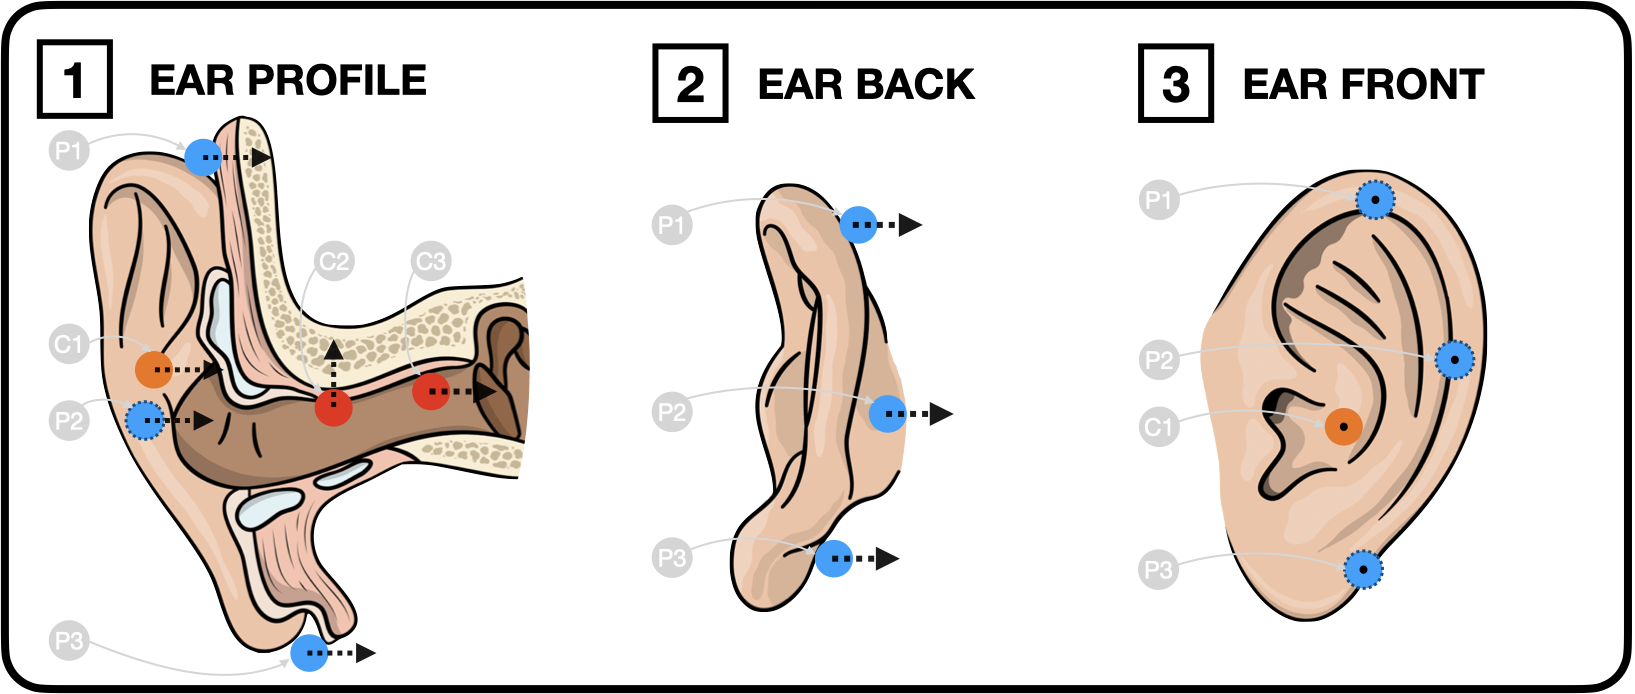
\includegraphics[scale=0.26]{thesis-doc/images/ear_measurement_points/emp.png}
    \caption{Here the temperature measurement points are shown visually from different angles (profile view (1), ear from behind (2), ear from the side (3)). $P1$-$P3$ are three measuring points behind the ear, which measure the skin temperature at the mastoid. $C1$ is a measuring point that measures the temperature at the concha. $C2$ and $C3$ measure the temperature in the ear canal, where $C3$ is directed at the tympanic membrane and $C2$ is directed at the edge of the ear canal. The arrows at each measuring point show the measuring direction. In addition, a measuring point is outlined with a dashed line if it is located behind the ear. The sensor used is the MLX90632, which is an infrared temperature sensor. This is connected to the OpenEarable and the sensor values can be received and persisted using the I2C protocol.}
    \label{fig:ear_measurement_positions}
\end{figure}

In order to position the temperature sensors at the selected positions and to record the temperature values with them, a prototype is built for this master thesis.
Subsequently, two studies will be conducted, the first of which will look at and compare the positions and the second of which will compare the temperature behavior under stress at the different sensor positions.

The OpenEarable platform is used as a basis, which makes it possible to attach various temperature sensors to the ear canal in an uncomplicated manner. 
The sensors are placed at various locations, including the concha, inside the ear canal, at a location facing the tympanic membrane, and behind the concha.
The exact locations can be explored in Figure \ref{fig:ear_measurement_positions}.
Two circuit boards will be designed for this purpose, furthermore a case for comfortable wearing during the study.
Participants will be asked to wear the sensors in a study under similar conditions on the right ear.
The resulting data will be collected and then analyzed to compare sensor positions for ear-based temperature measurement. 
These positions will then be used to classify body stress induced in the second study based on body temperature.
To gain additional insights, it is planned to perform temperature measurements during different activities in a first study to see how the measurements behave in different situations. 
In addition, it is planned to conduct a second study to observe the temperature readings at the different sensor locations under stress.
This results in two independent studies from which the following hypotheses emerge:

\textbf{Study 1}
\begin{enumerate}[label=H\arabic{*}:]
  \item The temperature measured by sensors located behind the ear is lower compared to the other locations.
  \item The variance in temperature readings differs between indoor and outdoor settings.
  \item Relative changes in temperature readings across different sensor locations will be interrelated.
  \item The temperature at the tympanic membrane has the greatest stability compared to other sensor locations.
  \item Subject movement leads to significant changes in the temperature readings across various sensor locations.
\end{enumerate}

\textbf{Study 2}
\begin{enumerate}[label=H\arabic{*}:]
  \item A measurable rise in temperature occurs during stress-inducing activities.
  \item There will be variability in temperature changes across different types of stress tests.
\end{enumerate}

\section{Expected Results}
\label{ch:Introduction:ExpectedResults}
The study is expected to provide insights into the placement of sensors for temperature monitoring in or directly on the ear.
Possible variations in temperature measurements at different positions in the ear canal will be identified to adequately detect temperature at the ear in everyday situations.
The results will support the development of more accurate and reliable wearable devices for biometric applications. 
In addition, the optimally determined position will serve as a new basis for the analysis of various body temperature changing events.
The second study, which is being conducted as part of this work, will demonstrate small-scale temperature increases under stress and provide preliminary findings.